
正则表达式(通常缩写为regex)通常用于文本流的词法分析和模式匹配。它们在Unix文本处理实用程序(如grep、awk和sed)中很常见,并且是Perl语言不可分割的一部分。POSIX标准于1992年获得批准,而其他常见的变体包括Perl和ECMAScript (JavaScript)方言。C++ regex库默认使用ECMAScript方言。

regex库是在C++11中首次引入STL的,其对于在文本文件中查找模式非常有用。

要了解更多关于正则表达式的语法和用法,我推荐Jeffrey Friedl的《Mastering Regular Expressions》这本书。

\subsubsection{How to do it…}

对于这个示例,我们将从HTML文件中提取超链接。超链接是这样用HTML编码的:

\begin{lstlisting}[style=styleCXX]
<a href="http://example.com/file.html">Text goes here</a>
\end{lstlisting}

我们将使用一个regex对象来提取链接和文本,作为两个单独的字符串。


\begin{itemize}
\item 
我们的示例文件名为the-end.html。它来自我的网站(\url{https://bw.org/end/}),并包含在GitHub存储库中:

\begin{lstlisting}[style=styleCXX]
const char *fn{ "the-end.html" };
\end{lstlisting}

\item 
现在,用正则表达式字符串定义regex对象:

\begin{lstlisting}[style=styleCXX]
const std::regex
	link_re{ "<a href=\"([^\"]*)\"[^<]*>([^<]*)</a>" };
\end{lstlisting}

正则表达式一开始看起来很吓人,但实际上它们很简单。

解析如下:

\begin{enumerate}[label=\Roman*.]
\item 
匹配整个字符串。

\item 
查找子字符串<a href="

\item 
存储到下一个双引号间的所有内容,作为子匹配1。

\item 
跳过>字符。

\item 
将字符串</a>之前的所有内容存储为子匹配2。
\end{enumerate}

\item 
现在,将文件放入一个字符串:

\begin{lstlisting}[style=styleCXX]
string in{};
std::ifstream infile(fn, std::ios_base::in);
for(string line{}; getline(infile, line);) in += line;
\end{lstlisting}

这将打开HTML文件,逐行读取它,并将每行追加到字符串对象中。

\item 
为了提取链接字符串,设置了sregex\_token\_iterator对象,来逐级遍历文件并提取每个匹配的元素:

\begin{lstlisting}[style=styleCXX]
std::sregex_token_iterator it{ in.begin(), in.end(),
	link_re, {1, 2} };
\end{lstlisting}

1和2对应正则表达式中的子匹配项。

\item 
我们有一个对应的函数,用迭代器逐级遍历结果:

\begin{lstlisting}[style=styleCXX]
template<typename It>
void get_links(It it) {
	for(It end_it{}; it != end_it; ) {
		const string link{ *it++ };
		if(it == end_it) break;
		const string desc{ *it++ };
		cout << format("{:.<24} {}\n", desc, link);
	}
}
\end{lstlisting}

使用regex迭代器调用函数:

\begin{lstlisting}[style=styleCXX]
get_links(it);
\end{lstlisting}

用描述和链接得到了这个结果:

\begin{tcblisting}{commandshell={}}
Bill Weinman............ https://bw.org/
courses................. https://bw.org/courses/
music................... https://bw.org/music/
books................... https://packt.com/
back to the internet.... https://duckduckgo.com/
\end{tcblisting}
\end{itemize}

\subsubsection{How it works…}

STL正则表达式引擎作为生成器运行,每次计算并产生一个结果。我们使用sregex\_iterator或sregex\_token\_iterator来设置迭代器,sregex\_token\_iterator支持子匹配,sregex\_iterator不支持子匹配。

正则表达式中的括号作为子匹配项,分别编号为1和2:

\begin{lstlisting}[style=styleCXX]
const regex link_re{ "<a href=\"([^\"]*)\"[^<]*>([^<]*)</a>" };
\end{lstlisting}

正则表达式匹配的每个部分如下图所示:

\begin{center}
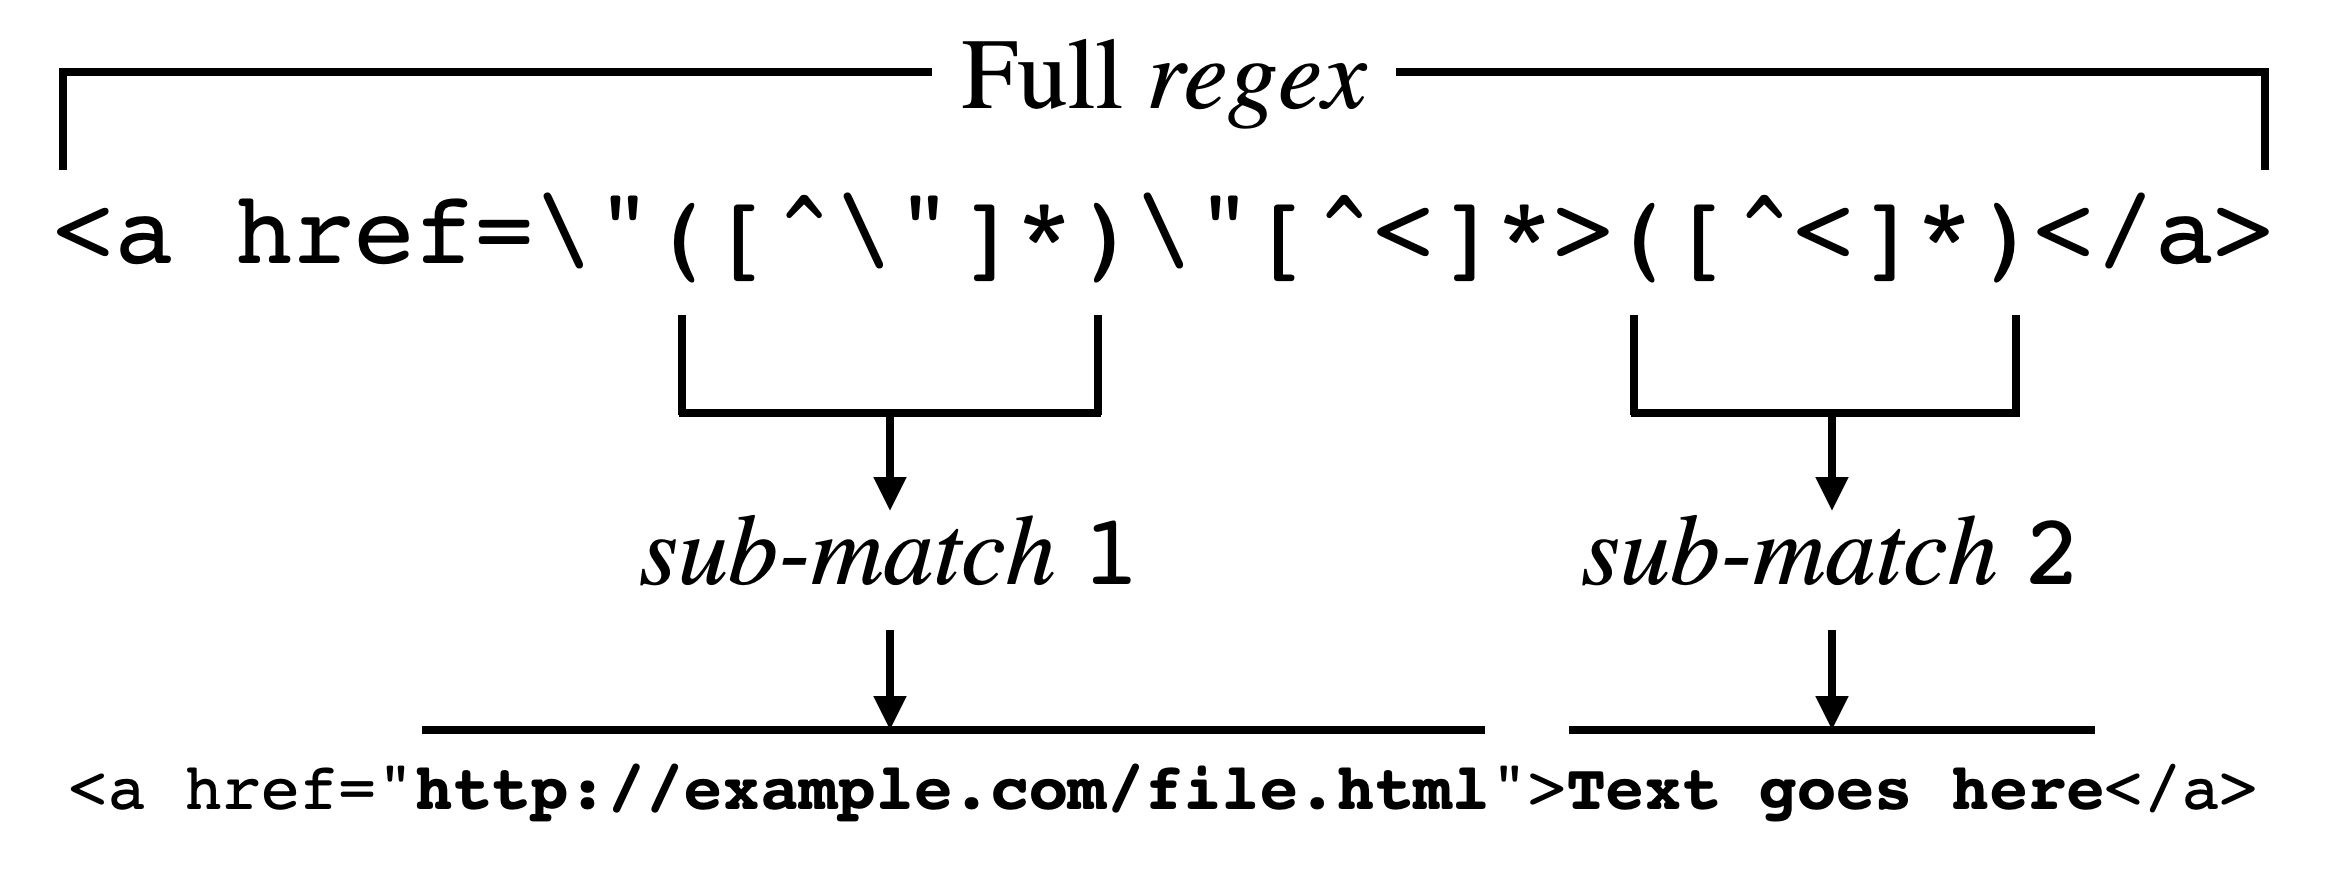
\includegraphics[width=0.8\textwidth]{content/chapter7/images/1.png}\\
图7.1 带有子匹配项的正则表达式
\end{center}

这允许我们匹配一个字符串,并使用该字符串的部分作为的结果:

\begin{lstlisting}[style=styleCXX]
sregex_token_iterator it{ in.begin(), in.end(), link_re, {1, 2}
};
\end{lstlisting}

子匹配项从1开始编号。子匹配0是一个特殊值,表示整个匹配。

要支持迭代器,就可以像这样使用:

\begin{lstlisting}[style=styleCXX]
for(It end_it{}; it != end_it; ) {
	const string link{ *it++ };
	if(it == end_it) break;
	const string desc{ *it++ };
	cout << format("{:.<24} {}\n", desc, link);
}
\end{lstlisting}

这只是通过regex迭代器逐步遍历结果,格式化的输出如下所示:

\begin{tcblisting}{commandshell={}}
Bill Weinman............ https://bw.org/
courses................. https://bw.org/courses/
music................... https://bw.org/music/
books................... https://packt.com/
back to the internet.... https://duckduckgo.com/
\end{tcblisting}












